\documentclass[a4paper,11pt,oneside]{memoir}

% Castellano
\usepackage[spanish,es-tabla]{babel}
\selectlanguage{spanish}
\usepackage[utf8]{inputenc}
\usepackage{placeins}
\usepackage{float}

\RequirePackage{booktabs}
\RequirePackage[table]{xcolor}
\RequirePackage{xtab}
\RequirePackage{multirow}

% Multi-page tables using
\usepackage{longtable}
\usepackage{tabularx}

% Cell with line break (e.g. \specialcell{Foo\\bar})
\newcommand{\specialcell}[2][c]{%
  \begin{tabular}[#1]{@{}l@{}}#2\end{tabular}}

% Mathematic font
\usepackage{amsfonts}

% Color

% Bibliography management
\usepackage[numbers,sort]{natbib}

% Links
\usepackage[colorlinks]{hyperref}
\hypersetup{
	colorlinks,
	linkcolor={green!40!black},
	citecolor={blue!50!black},
	urlcolor={blue!80!black}
}

% Ecuaciones
\usepackage{amsmath}

% Rutas de fichero / paquete
\newcommand{\ruta}[1]{{\sffamily #1}}

% Párrafos
\nonzeroparskip

% Listas estrechas
\providecommand{\tightlist}{%
  \setlength{\itemsep}{0pt}\setlength{\parskip}{0pt}}

% Imagenes
\usepackage{graphicx}
\newcommand{\imagen}[2]{
	\begin{figure}[!h]
		\centering
		\includegraphics[width=0.9\textwidth]{#1}
		\caption{#2}\label{fig:#1}
	\end{figure}
	\FloatBarrier
}

\newcommand{\imagenflotante}[2]{
	\begin{figure}%[!h]
		\centering
		\includegraphics[width=0.9\textwidth]{#1}
		\caption{#2}\label{fig:#1}
	\end{figure}
}



% El comando \figura nos permite insertar figuras comodamente, y utilizando
% siempre el mismo formato. Los parametros son:
% 1 -> Porcentaje del ancho de página que ocupará la figura (de 0 a 1)
% 2 --> Fichero de la imagen
% 3 --> Texto a pie de imagen
% 4 --> Etiqueta (label) para referencias
% 5 --> Opciones que queramos pasarle al \includegraphics
% 6 --> Opciones de posicionamiento a pasarle a \begin{figure}
\newcommand{\figuraConPosicion}[6]{%
  \setlength{\anchoFloat}{#1\textwidth}%
  \addtolength{\anchoFloat}{-4\fboxsep}%
  \setlength{\anchoFigura}{\anchoFloat}%
  \begin{figure}[#6]
    \begin{center}%
      \Ovalbox{%
        \begin{minipage}{\anchoFloat}%
          \begin{center}%
            \includegraphics[width=\anchoFigura,#5]{#2}%
            \caption{#3}%
            \label{#4}%
          \end{center}%
        \end{minipage}
      }%
    \end{center}%
  \end{figure}%
}

%
% Comando para incluir imágenes en formato apaisado (sin marco).
\newcommand{\figuraApaisadaSinMarco}[5]{%
  \begin{figure}%
    \begin{center}%
    \includegraphics[angle=90,height=#1\textheight,#5]{#2}%
    \caption{#3}%
    \label{#4}%
    \end{center}%
  \end{figure}%
}
% Para las tablas
\newcommand{\otoprule}{\midrule [\heavyrulewidth]}
%
% Nuevo comando para tablas pequeñas (menos de una página).
\newcommand{\tablaSmall}[5]{%
 \begin{table}[H]
  \begin{center}
   \rowcolors {2}{gray!35}{}
   \begin{tabular}{#2}
    \toprule
    #4
    \otoprule
    #5
    \bottomrule
   \end{tabular}
   \caption{#1}
   \label{tabla:#3}
  \end{center}
 \end{table}
}

%
% Nuevo comando para tablas pequeñas (menos de una página).
\newcommand{\tablaSmallSinColores}[5]{%
 \begin{table}[H]
  \begin{center}
   \begin{tabular}{#2}
    \toprule
    #4
    \otoprule
    #5
    \bottomrule
   \end{tabular}
   \caption{#1}
   \label{tabla:#3}
  \end{center}
 \end{table}
}

\newcommand{\tablaApaisadaSmall}[5]{%
\begin{landscape}
  \begin{table}
   \begin{center}
    \rowcolors {2}{gray!35}{}
    \begin{tabular}{#2}
     \toprule
     #4
     \otoprule
     #5
     \bottomrule
    \end{tabular}
    \caption{#1}
    \label{tabla:#3}
   \end{center}
  \end{table}
\end{landscape}
}

%
% Nuevo comando para tablas grandes con cabecera y filas alternas coloreadas en gris.
\newcommand{\tabla}[6]{%
  \begin{center}
    \tablefirsthead{
      \toprule
      #5
      \otoprule
    }
    \tablehead{
      \multicolumn{#3}{l}{\small\sl continúa desde la página anterior}\\
      \toprule
      #5
      \otoprule
    }
    \tabletail{
      \hline
      \multicolumn{#3}{r}{\small\sl continúa en la página siguiente}\\
    }
    \tablelasttail{
      \hline
    }
    \bottomcaption{#1}
    \rowcolors {2}{gray!35}{}
    \begin{xtabular}{#2}
      #6
      \bottomrule
    \end{xtabular}
    \label{tabla:#4}
  \end{center}
}

%
% Nuevo comando para tablas grandes con cabecera.
\newcommand{\tablaSinColores}[6]{%
  \begin{center}
    \tablefirsthead{
      \toprule
      #5
      \otoprule
    }
    \tablehead{
      \multicolumn{#3}{l}{\small\sl continúa desde la página anterior}\\
      \toprule
      #5
      \otoprule
    }
    \tabletail{
      \hline
      \multicolumn{#3}{r}{\small\sl continúa en la página siguiente}\\
    }
    \tablelasttail{
      \hline
    }
    \bottomcaption{#1}
    \begin{xtabular}{#2}
      #6
      \bottomrule
    \end{xtabular}
    \label{tabla:#4}
  \end{center}
}

%
% Nuevo comando para tablas grandes sin cabecera.
\newcommand{\tablaSinCabecera}[5]{%
  \begin{center}
    \tablefirsthead{
      \toprule
    }
    \tablehead{
      \multicolumn{#3}{l}{\small\sl continúa desde la página anterior}\\
      \hline
    }
    \tabletail{
      \hline
      \multicolumn{#3}{r}{\small\sl continúa en la página siguiente}\\
    }
    \tablelasttail{
      \hline
    }
    \bottomcaption{#1}
  \begin{xtabular}{#2}
    #5
   \bottomrule
  \end{xtabular}
  \label{tabla:#4}
  \end{center}
}



\definecolor{cgoLight}{HTML}{EEEEEE}
\definecolor{cgoExtralight}{HTML}{FFFFFF}

%
% Nuevo comando para tablas grandes sin cabecera.
\newcommand{\tablaSinCabeceraConBandas}[5]{%
  \begin{center}
    \tablefirsthead{
      \toprule
    }
    \tablehead{
      \multicolumn{#3}{l}{\small\sl continúa desde la página anterior}\\
      \hline
    }
    \tabletail{
      \hline
      \multicolumn{#3}{r}{\small\sl continúa en la página siguiente}\\
    }
    \tablelasttail{
      \hline
    }
    \bottomcaption{#1}
    \rowcolors[]{1}{cgoExtralight}{cgoLight}

  \begin{xtabular}{#2}
    #5
   \bottomrule
  \end{xtabular}
  \label{tabla:#4}
  \end{center}
}


















\graphicspath{ {../img/} }

% Capítulos
\chapterstyle{bianchi}
\newcommand{\capitulo}[2]{
	\setcounter{chapter}{#1}
	\setcounter{section}{0}
	\chapter*{#2}
	\addcontentsline{toc}{chapter}{#2}
	\markboth{#2}{#2}
}

% Apéndices
\renewcommand{\appendixname}{Apéndice}
\renewcommand*\cftappendixname{\appendixname}

\newcommand{\apendice}[1]{
	%\renewcommand{\thechapter}{A}
	\chapter{#1}
}

\renewcommand*\cftappendixname{\appendixname\ }

% Formato de portada
\makeatletter
\usepackage{xcolor}
\newcommand{\tutor}[1]{\def\@tutor{#1}}
\newcommand{\course}[1]{\def\@course{#1}}
\definecolor{cpardoBox}{HTML}{E6E6FF}
\def\maketitle{
  \null
  \thispagestyle{empty}
  % Cabecera ----------------
\noindent
\includegraphics[width=\textwidth]{cabecera}\vspace{1cm}%
  \vfill
  % Título proyecto y escudo informática ----------------
  \colorbox{cpardoBox}{%
    \begin{minipage}{.8\textwidth}
      \vspace{.5cm}\Large
      \begin{center}
      \textbf{TFG del Grado en Ingeniería Informática}\vspace{.6cm}\\
      \textbf{\LARGE\@title{}}
      \end{center}
      \vspace{.2cm}
    \end{minipage}

  }%
  \hfill\begin{minipage}{.20\textwidth}
    \includegraphics[width=\textwidth]{escudoInfor}
  \end{minipage}
  \vfill
  % Datos de alumno, curso y tutores ------------------
  \begin{center}%
  {%
    \noindent\LARGE
    Presentado por \@author{}\\ 
    en la Universidad de Burgos --- \@date{}\\
    Tutores: \@tutor{}\\
  }%
  \end{center}%
  \null
  \cleardoublepage
  }
\makeatother

\newcommand{\nombre}{David Miguel Lozano} %%% cambio de comando

% Datos de portada
\title{{\Huge GoBees}\\[0.5cm]Monitorización del estado de una colmena mediante la cámara de un smartphone.}
\author{\nombre}
\tutor{Dr. José Francisco Díez Pastor\\y Dr. Raúl Marticorena Sánchez}
\date{\today}

\begin{document}

\maketitle



\newpage\null\thispagestyle{empty}\newpage


%%%%%%%%%%%%%%%%%%%%%%%%%%%%%%%%%%%%%%%%%%%%%%%%%%%%%%%%%%%%%%%%%%%%%%%%%%%%%%%%%%%%%%%%
\thispagestyle{empty}


\noindent
\includegraphics[width=\textwidth]{cabecera}\vspace{1cm}

\noindent D. José Francisco Díez Pastor y D. Raúl Marticorena Sánchez, profesores del departamento de Ingeniería Civil, área de Lenguajes y Sistemas Informáticos.

\noindent Exponen:

\noindent Que el alumno D. \nombre, con DNI 71307412Y, ha realizado el Trabajo Final de Grado en Ingeniería Informática titulado ``GoBees - Monitorización del estado de una colmena mediante la cámara de un smartphone''. 

\noindent Y que dicho trabajo ha sido realizado por el alumno bajo la dirección del que suscribe, en virtud de lo cual se autoriza su presentación y defensa.

\begin{center} %\large
En Burgos, {\large \today}
\end{center}

\vfill\vfill\vfill

% Author and supervisor
\begin{minipage}{0.45\textwidth}
\begin{flushleft} %\large
Vº. Bº. del Tutor:\\[2cm]
D. José Francisco Díez Pastor
\end{flushleft}
\end{minipage}
\hfill
\begin{minipage}{0.45\textwidth}
\begin{flushleft} %\large
Vº. Bº. del Tutor:\\[2cm]
D. Raúl Marticorena Sánchez
\end{flushleft}
\end{minipage}
\hfill

\vfill

% para casos con solo un tutor comentar lo anterior
% y descomentar lo siguiente
%Vº. Bº. del Tutor:\\[2cm]
%D. nombre tutor


\newpage\null\thispagestyle{empty}\newpage




\frontmatter

% Abstract en castellano
\renewcommand*\abstractname{Resumen}
\begin{abstract}
La actividad de vuelo de una colmena es un indicador importante sobre su
estado de salud. Sin embargo, la monitorización manual de este parámetro
es un proceso muy costoso y puede introducir una tasa de error elevada.
Por ello, se han desarrollado diversos métodos que permiten automatizar
este proceso.

En este trabajo se propone un nuevo método más accesible al público
general que permite la monitorización de la actividad de vuelo de una
colmena mediante la cámara de un \emph{smartphone} Android.

Además, se ha desarrollado una aplicación de gestión de colmenares que
integra el algoritmo y proporciona las herramientas necesarias para
interpretar y organizar toda la información recabada.

GoBees es la aplicación resultante y se encuentra disponible a través de
Google Play o de la página oficial del proyecto \url{http://gobees.io/}.
\end{abstract}

\renewcommand*\abstractname{Descriptores}
\begin{abstract}
Contador de abejas, actividad de vuelo, monitorización de colmenas, 
gestión de colmenares, aplicación Android.
\end{abstract}

\clearpage

% Abstract en inglés
\renewcommand*\abstractname{Abstract}
\begin{abstract}
Flight activity of a honey bee colony is an overall indicator of the
state of the hive's health. However, manually monitoring this parameter
is a very expensive and time-consuming process and can introduce a high
error rate. Thus, several methods to automate this process have been
developed over the years.

In this work, we propose a new method more accessible to the general
public which allows monitoring the flight activity of a honey bee colony
using the built-in camera of an Android smartphone.

In addition, an apiary management application has been developed,
incorporating the algorithm and providing the necessary tools to
interpret and organize all the information gathered.

GoBees is the resulting application and it is available from Google Play
or the official web site \url{http://gobees.io/}.
\end{abstract}

\renewcommand*\abstractname{Keywords}
\begin{abstract}
Bee counter, flight activity, hive monitoring, apiary management, 
Android application.
\end{abstract}

\clearpage

% Indices
\tableofcontents

\clearpage

\listoffigures

\clearpage

%\listoftables

%\clearpage

\mainmatter
\include{./tex/1_Introduccion}
\include{./tex/2_Objetivos_del_proyecto}
\capitulo{3}{Conceptos teóricos}

La parte del proyecto con mayor complejidad teórica radica en el
algoritmo de visión artificial, el cual se puede dividir en cuatro
fases. En primer lugar, se realiza un preprocesado de la señal de
entrada para optimizarla. En segundo lugar, se substrae el fondo para
segmentar los objetos en movimiento. Posteriormente, se realiza un
posprocesado de la señal para mejorar los resultados obtenidos de la
substracción del fondo. Y por último, se clasifican y cuentan los
contornos que pueden pertenecer a una abeja.

A continuación se exponen los conceptos teóricos que conlleva cada fase.

\section{Preprocesado}\label{preprocesado}

Antes de aplicar el algoritmo de substracción del fondo, es recomendable
realizar un preprocesado de los fotogramas para facilitar el procesado
posterior, minimizar el ruido y optimizar los resultados. A continuación
se explican las técnicas utilizadas.

\subsection{Conversión de RGB a escala de grises}\label{conversion-de-rgb-a-escala-de-grises}

Los fotogramas captados por la cámara se devuelven en formato RGB. En
este formato se poseen tres matrices, una por cada canal
(\emph{Red-Green-Blue}). La suma aditiva de los tres canales resulta en
una imagen a color.

Sin embargo, el color no proporciona ninguna información relevante en
nuestra tarea de identificación de abejas. Es por esto que se pueden
convertir los fotogramas de RGB a escala de grises. De esta manera, se
trabajará solamente con una matriz de píxeles en lugar de tres.
Simplificando, en gran medida, el número de operaciones a realizar y por
tanto, aumentado el rendimiento de nuestro algoritmo final.

OpenCV utiliza la conversión colométrica a escala de grises
\citep{opencv:color_cvt}. Esta técnica se basa en principios
colométricos para ajustar la luminancia de la imagen a color y la imagen
resultante. Devolviendo una imagen con la misma luminancia absoluta y la
misma percepción de luminosidad \citep{wiki:grayscale}.

Utiliza la siguiente fórmula para calcular la luminancia resultante:

\begin{equation*}
    \text{RGB[A] to Gray:} \quad Y \leftarrow 0.299 \cdot R + 0.587 \cdot G + 0.114 \cdot B
\end{equation*}

La fórmula calcula la luminancia de una forma no lineal, sin necesidad
de realizar una expansión gamma. Los coeficientes intentan imitar la
percepción de intensidad medida por un humano tricromático, siendo más
sensible al color verde y menos al color azul \citep{wiki:grayscale}.

\subsection{Desenfoque Gaussiano}\label{desenfoque-gaussiano}

Las imágenes captadas pueden contener ruido que puede dificultar su
procesamiento. El ruido son variaciones aleatorias del brillo o del
color de una imagen. Una técnica que permite reducirlo es el desenfoque.

En nuestro caso hemos utilizado desenfoque Gaussiano, un filtro de paso
bajo que reduce las componentes de alta frecuencia de la imagen
utilizando para ello una convolución con una función Gaussiana
\citep{wiki:gaussian}. Se diferencia del desenfoque promedio en que da
más peso a los vecinos cercanos, siendo estos más influyentes en el
resultado.

El kernel utilizado en la convolución es una muestra discreta de una
función Gaussiana. En nuestro caso utilizamos un kernel 3x3 que se
corresponde con: \citep{book:mastering_opencv}

\begin{equation*}
    M = 
    \begin{bmatrix}
    1 & 2 & 1 \\[0.3em] 
    2 & 4 & 2 \\[0.3em] 
    1 & 2 & 1
    \end{bmatrix}
\end{equation*}

En la siguiente imagen se puede ver el resultado de aplicar esta fase a
la imagen de entrada:

\imagen{s1}{Resultado de la fase de preprocesado.}

\section{Substracción del fondo}\label{substraccion-del-fondo}

En un sistema de monitorización por vídeo resulta de gran interés el
poder extraer los objetos en movimiento del resto de la imagen. Esto se
conoce como extracción del fondo, en inglés \emph{background
subtraction} o \emph{foreground detection}, y consiste en clasificar
todos los píxeles de un determinado fotograma bien como fondo, o como
primer plano \citep{wiki:bs}. En primer plano se engloban todos los
objetos en movimiento, mientras que en el fondo se encuentran todos los
objetos estáticos junto con posibles sombras, cambios de iluminación u
otros objetos en movimiento que no son de interés, como puede ser la
rama de un árbol balanceándose por el viento. Se trata de un paso
crítico, ya que algoritmos posteriores dependen en gran medida de los
resultados de este.

En nuestro proyecto, la toma de imágenes se realiza mediante una cámara
estática. Esto facilita en parte la detección del fondo, ya que este se
corresponderá con todos los píxeles estáticos. Sin embargo, como
trabajamos en un entorno al aire libre, tenemos que lidiar también con
cambios de iluminación, sombras, u otros objetos móviles que no son de
nuestro interés (falsos positivos).

Con OpenCV para Android podemos implementar varios algoritmos básicos de
extracción del fondo y además, nos proporciona la implementación de dos
algoritmos más sofisticados: \texttt{BackgroundSubtractorMOG} y \\
\texttt{BackgroundSubtractorKNN}. 

Tras realizar un estudio de todos
ellos, nos decantamos finalmente por \texttt{BackgroundSubtractorMOG2}.
A continuación, explicamos el funcionamiento de todos los algoritmos que
se probaron, así como los resultados que proporcionaron.

\subsection{Substracción con imagen de referencia}\label{substraccion-con-imagen-de-referencia}

Se parte de una imagen de referencia del fondo, en la que no haya ningún
objeto en movimiento. A partir de esta, se obtienen los elementos en
movimiento substrayendo a cada fotograma la imagen tomada como
referencia.

Este método, al tomar un modelo del fondo tan sencillo y estático, es
muy vulnerable a cambios en la escena (iluminación, sombras, objetos del
fondo con ligeros movimientos, pequeñas oscilaciones de la cámara,
etc.). Sin embargo, ofrece muy buenos resultados cuando se trabaja en
una escena con la iluminación y los elementos controlados, ya que al ser
tan simple, es muy eficiente \citep{programarfacil:detmov}.

Para implementar este algoritmo con OpenCV, se hace uso de la función
\texttt{Core.absdiff()}.

En nuestro problema, al trabajar al aire libre nos es imposible utilizar
este algoritmo. Ya que el modelo del fondo cambia constantemente.

\subsection{Substracción del fotograma anterior}\label{substraccion-del-fotograma-anterior}

En este método, el modelo del fondo se extrae del fotograma anterior. De
tal manera, que a cada nuevo fotograma se le substrae el anterior.

De esta manera se mejora la respuesta a cambios en la escena, como los
cambios de iluminación. Sin embargo, si un objeto en movimiento se queda
estático en la imagen, este deja de ser detectado
\citep{book:opencv_java}.

La implementación se realiza como en la técnica anterior, variando el
modelo del fondo.

Tras probarlo en nuestro problema específico, vimos que no nos era de
utilidad. Ya que el fotograma resultante de la diferencia contenía las
abejas por duplicado (la abeja en el fotograma actual y misma abeja en
el fotograma anterior en otra posición).

\subsection{Substracción del acumulado de los fotogramas anteriores}\label{substraccion-del-acumulado-de-los-fotogramas-anteriores}

Una mejora interesante del algoritmo anterior supone tomar como modelo
del fondo un acumulado de los fotogramas anteriores de acuerdo a un
ratio de aprendizaje. De esta forma, se puede lidiar con cambios en el
fondo de la imagen dinámicamente. El modelo se calcula de acuerdo a la
siguiente fórmula:

\begin{equation*}
    u_t = (1-\alpha )u_{t-1}+\alpha\ p_t
\end{equation*}

Donde $p_t$ es el nuevo valor del píxel, $u_{t-1}$ es la media del
fondo en el instante $t-1$, $u_t$ es la nueva media del fondo y
$\alpha$ es el ratio de aprendizaje (cómo de rápido olvida los \emph{frames}
anteriores) \citep{book:opencv_java}.

OpenCV provee la función \texttt{Imgproc.accumulateWeighted()} que
implementa la fórmula anterior por nosotros. Haciendo uso de esta
función y de la utilizada en la sección anterior podemos implementar
este algoritmo.

Tras probarlo, vimos que tenía una eficiencia muy buena y se adaptaba a
los cambios correctamente. Sin embargo, no era capaz de diferenciar las
sombras de las abejas, por lo que se obtenían falsos positivos.

\subsection{BackgroundSubtractorKNN}\label{backgroundsubtractorknn}

Se trata de un método que se basa en el algoritmo de clasificación
supervisada \emph{K Nearest Neighbors} (k-nn). El algoritmo fue
propuesto en el artículo \citep{art:zivkovic_efficient_2006}. Y de
acuerdo con sus conclusiones, es muy eficiente cuando el número de
píxeles que se corresponden con el primer plano es bajo.

La clase de OpenCV que lo implementa es
\texttt{BackgroundSubtractorKNN}. Los parámetros más importantes son:

\begin{itemize}
\tightlist
\item
  \texttt{history}: número de fotogramas recientes que afectan al modelo
  del fondo.
\item
  \texttt{dist2Threshold}: umbral de la distancia al cuadrado entre el
  píxel y la muestra para decidir si un píxel está cerca de esa muestra.
\item
  \texttt{detectShadows}: con un valor verdadero detecta las sombras
  (aumenta considerablemente el tiempo de procesado).
\end{itemize}

En nuestras pruebas, el algoritmo proporcionaba unos resultados buenos
pero su tiempo de ejecución era muy elevado (entorno a 25ms/frame). Como
el tiempo de ejecución es un factor clave en nuestro proyecto, se
descartó el uso de este algoritmo.

\subsection{BackgroundSubtractorMOG2}\label{backgroundsubtractormog2}

\texttt{BackgroundSubtractorMOG2} es una mejora del algoritmo
\\ \texttt{BackgroundSubtractorMOG}. En la versión original de OpenCV se
encuentran implementados ambos, sin embargo, en los \emph{wrappers} para
Android solo disponemos de la revisión.

\texttt{BackgroundSubtractorMOG} está basado en el modelo \emph{Gaussian
Mixture} (GMM). Se trata de un modelo compuesto por la suma de varias
distribuciones Gaussianas que, correctamente elegidas, permiten modelar
cualquier distribución \citep{coursera:gmm}.

El algoritmo de substracción del fondo fue propuesto en el artículo
\citep{art:yao_improved_2001} y modela cada píxel del fondo como la
mezcla de \emph{K} distribuciones Gaussianas. Los pesos de la mezcla
representan las proporciones de tiempo que el color de ese píxel se ha
mantenido en la escena. Siendo los colores de fondo más probables los
que más permanezcan y sean más estáticos \citep{opencv:bs_tutorial}.

\texttt{BackgroundSubtractorMOG2} se basa en los mismos principios que
su antecesor pero implementa una mejora sustancial. Es el propio
algoritmo el que selecciona el número adecuado de distribuciones
Gaussianas necesarias para modelar cada píxel. De esta manera, se mejora
notablemente la adaptabilidad del algoritmo a variaciones en la escena.
Fue propuesto en los artículos \citep{art:zivkovic_improved_2004} y
\citep{art:zivkovic_efficient_2006}.

El código fuente de este algoritmo está disponible en 
\citep{github:background_segm} (interfaz) y
\citep{github:bgfg_gaussmix2} (implementación).

La clase de OpenCV que lo implementa es
\texttt{BackgroundSubtractorMOG2}. Posee los siguientes parámetros
configurables: \citep{opencv:mog2}

\begin{itemize}
\tightlist
\item
  \texttt{history}: número de fotogramas recientes que afectan al modelo
  del fondo. Se representa en la literatura como \texttt{T}. Por
  defecto, 500 fotogramas. Nosotros hemos obtenido buenos resultados con
  valores de entorno a 50.
\item
  \texttt{learningRate}: valor entre 0 y 1 que indica como de rápido
  aprende el modelo. Si se establece un valor de -1 el algoritmo elige
  automáticamente el ratio. 0 significa que el modelo del fondo no se
  actualiza para nada, mientras que 1 supone que el modelo del fondo se
  reinicializa completamente cada nuevo fotograma. En la literatura
  podemos encontrar este parámetro como \texttt{alfa}. Si el intervalo
  que se quiere considerar es \texttt{history}, se debe establecer
  \texttt{alfa=1/history} (valor por defecto). También se pueden mejorar
  los resultados iniciales estableciendo \texttt{alfa=1} en el instante
  0 e ir decrementándolo hasta \texttt{alfa=1/history}. De esta manera,
  en el inicio aprende rápidamente, pero una vez estabilizada la
  situación las variaciones afectan menos al modelo. En nuestro caso, el
  valor por defecto ha funcionado correctamente.
\item
  \texttt{backgroundRatio}: si un pixel del primer plano permanece con
  un valor semi-constante durante \texttt{backgroundRatio*history}
  fotogramas, es considerado fondo y se añade al modelo del fondo como
  centro de una nueva componente Gaussiana. En los artículos se hace
  referencia a este parámetro como \texttt{TB}. \texttt{TB=0.9} es el
  valor por defecto. Este parámetro nos permite decidir cuando dejar de
  contar una abeja que se ha quedado inmóvil o un objeto nuevo en la
  escena como podría ser una hoja que se acaba de caer de un árbol.
\item
  \texttt{detectShadows}: con un valor verdadero (valor por defecto)
  detecta las sombras (aumenta ligeramente el tiempo de procesado). Nos
  permite despreciar las sombras de las abejas con muy buenos
  resultados.
\item
  \texttt{shadowThreshold}: el algoritmo detecta las sombras comprobando
  si un píxel es una versión oscurecida del fondo. Este parámetro define
  cómo de oscura puede ser la sombra como máximo. Por ejemplo, un valor
  de 0.5 (valor por defecto) significa que si un píxel es más del doble
  de oscuro, entonces no se considerará sombra. En los artículos se
  representa como \texttt{Tau}.
\item
  \texttt{shadowValue}: es el valor utilizado para marcar los píxeles de
  sombras en la máscara resultante. El valor por defecto es 127. En la
  máscara devuelta, un valor de 0 siempre se corresponde con un pixel
  del fondo, mientras que un valor de 255 con un píxel del primer plano.
\item
  \texttt{nMixtures}: número máximo de componentes Gaussianas para
  modelar el modelo del fondo. El número actual se determina
  dinámicamente para cada píxel. Hemos utilizado el valor por defecto,
  5.
\item
  \texttt{varThreshold}: umbral utilizado en el cálculo de la distancia
  cuadrada de Mahalanobis entre el píxel y el modelo del fondo para
  decidir si una muestra está bien descrita por el modelo o no. Este
  parámetro no afecta a la actualización del modelo del fondo. Se
  representa como \texttt{Cthr}. Por defecto, 16. Se han obtenido
  mejores resultados con valores de entorno a 40.
\item
  \texttt{varThresholdGen}: umbral sobre la distancia cuadrada de
  Mahalanobis entre el píxel y el modelo para ayudar a decidir si un
  píxel está cercano a alguna de las componentes del modelo. Si no es
  así, es considerado como primer plano o añadido como centro de una
  nueva componente (dependiendo del \texttt{backgroundRatio}). Se
  representa como \texttt{Tg} y su valor por defecto es 9. Un valor
  menor genera más componentes Gaussianas, mientras que un valor mayor
  genera menos.
\item
  \texttt{complexityReductionThreshold}: este parámetro define el número
  de muestras necesarias para probar que una componente existe. Se
  representa como \texttt{CT}. Su valor por defecto es \texttt{CT=0.05}.
  Si se establece su valor a 0 se obtiene un algoritmo similar al de
  Stauffer \& Grimson (no se reduce el número de componentes).
\item
  \texttt{varInit}: varianza inicial de cada componente Gaussiana.
  Afecta a la velocidad de adaptación. Se debe ajustar teniendo en
  cuenta la desviación estandar de las imágenes. Por defecto es 15.
\item
  \texttt{varMin}: varianza mínima. Por defecto, 4.
\item
  \texttt{varMax}: varianza máxima. Por defecto, \texttt{5*varInit}.
\end{itemize}

De todos ellos, los parámetros más importantes a ajustar son
\texttt{history} o \texttt{learningRate}, \texttt{varThreshold} y
\texttt{detectShadows}.

La parametrización correcta de este algoritmo es clave para su buen
funcionamiento. Por ello, durante las pruebas se integró en nuestra
aplicación de desarrollo, permitiendo variar todos estos parámetros en
tiempo real. De esta manera, se pudo elegir la mejor configuración para
nuestro problema concreto.

Una vez parametrizado correctamente, vimos como este algoritmo era el
que mejores resultados nos proporcionaba. Con un tiempo de ejecución en
nuestro equipo de pruebas de entorno a 4 ms/frame, mucho menor que el
proporcionado por \texttt{BackgroundSubtractorKNN}, de entorno a
25 ms/frame. El algoritmo detectaba correctamente las abejas, era
resistente al ruido, y además, era capaz de diferenciar una abeja de su
sombra. Por todos estos motivos, se seleccionó para la fase de
substracción del fondo.

En la siguiente imagen se puede ver el resultado de aplicar
\\ \texttt{BackgroundSubtractorMOG2} a la salida de la fase anterior:

\imagen{s2}{Resultado de la fase de substracción del fondo.}

Se puede apreciar como ha descartado correctamente las sombras en
movimiento de los árboles y se ha quedado únicamente con los objetos en
movimiento.

\section{Posprocesado}\label{posprocesado}

Para mejorar los resultados de la extracción de fondo y preparar la
imagen para la búsqueda de contornos, se han aplicado las siguientes
técnicas:

\subsection{Dilatación}\label{dilatacion}

Se trata de una operación morfológica por la cual se expanden las
regiones luminosas de una imagen. Esto se consigue mediante la
sustitución de cada píxel por el más brillante de los vecinos
considerados por el \emph{kernel} (matriz utilizada para la
convolución). De esta manera se consiguen unir las regiones de abejas
que podían haberse roto \citep{book:mastering_opencv}.

\subsection{Erosión}\label{erosion}

Se trata de la operación contraria a la anterior, expande las regiones
oscuras de la imagen. Para ello se coge el valor mínimo de los valores
considerados por el \emph{kernel} \citep{book:mastering_opencv}.

La dilatación nos permite reconstruir las abejas, pero también aumenta
su tamaño, aumentando el riesgo de solapamientos. Para evitar esto, se
vuelve a reducir el tamaño de estas mediante una erosión.

En nuestro algoritmo aplicamos tres operaciones morfológicas seguidas:

\begin{enumerate}
\def\labelenumi{\arabic{enumi}.}
\tightlist
\item
  \textbf{Erosión (3x3)}: elimina las piernas de las abejas.
\item
  \textbf{Dilatación (2x2)}: junta la cabeza de las abejas con su cuerpo
  que en numerosas ocasiones es separado durante la substracción de
  fondo.
\item
  \textbf{Erosión (3x3)}: recupera el tamaño inicial.
\end{enumerate}

A continuación podemos ver el resultado de esta fase:

\begin{figure}[H]
	\centering
	\includegraphics[width=0.9\textwidth]{s3}
	\caption{Resultado de la fase de posprocesado.}
	\label{fig:s3}
\end{figure}

\section{Detección y conteo de abejas}\label{deteccion-y-conteo-de-abejas}

El último paso que realiza nuestro algoritmo de visión artificial es
detectar cuáles de las regiones obtenidas en la fase anterior se
correponden con abejas. Para ello, se realiza una búsqueda de contornos
y se filtran por área.

Entendemos por contorno una línea curva que une todos los puntos
continuos del borde de una región de un mismo color o intensidad.

La salida de la fase anterior es una imagen binaria con los objetos en
movimiento en blanco y el fondo en negro. Por lo tanto, el objetivo de
esta fase es detectar todas las regiones blancas que puedan
corresponderse con una abeja.

OpenCV provee la función \texttt{Imgproc.findContours()} para realizar
la búsqueda de contornos. Esta toma una imagen binaria y devuelve una
lista con todos los contornos encontrados. Para entender la función se
necesita comprender una serie de conceptos: \citep{opencv:contours}

\begin{itemize}
\tightlist
\item
  \textbf{Jerarquía}: los contornos pueden ser independientes unos de
  otros, o poseer una relación padre-hijo cuando un contorno está dentro
  de otro. En la jerarquía se especifican las relaciones entre
  contornos.
\item
  \textbf{Modo de obtención del contorno}: define cómo se van a obtener
  los contornos en cuestión de jerarquía \citep{opencv:find_contours}.

  \begin{itemize}
  \tightlist
  \item
    \texttt{RETR\_LIST}: devuelve todos los contornos en una lista, sin
    ninguna información de jerarquía entre ellos.
  \item
    \texttt{RETR\_EXTERNAL}: devuelve todos los contornos externos. Si
    algún contorno tiene contornos hijo, estos son ignorados.
  \item
    \texttt{RETR\_CCOMP}: devuelve los contornos agrupados en dos
    niveles de jerarquía. Un primer nivel en el que se encuentran todos
    los contornos exteriores. Y un segundo nivel con los contornos
    correspondientes a agujeros en los primeros.
  \item
    \texttt{RETR\_TREE}: devuelve todos los contornos creando un árbol
    completo con la jerarquía.
  \end{itemize}
\item
  \textbf{Método de aproximación de los contornos}: define el método que
  utiliza la función para almacenar los contornos
  \citep{opencv:find_contours}.

  \begin{itemize}
  \tightlist
  \item
    \texttt{CHAIN\_APPROX\_NONE}: almacena todos los puntos del borde
    del contorno.
  \item
    \texttt{CHAIN\_APPROX\_SIMPLE}: almacena sólo los puntos relevantes
    del contorno. Por ejemplo, si el contorno es una línea no se
    necesita almacenar todos los puntos de esta, con el punto inicial y
    el final basta. Esto es lo que realiza este método, eliminar todos
    los puntos redundantes y comprimirlos para que ocupe menos espacio.
  \item
    \texttt{CV\_CHAIN\_APPROX\_TC89\_L1} y
    \texttt{CV\_CHAIN\_APPROX\_TC89\_KCOS}: aplican el algoritmo de
    aproximación de cadena de Teh-Chin, simplificando los polígonos que
    forman los contornos.
  \item
    \texttt{CV\_CHAIN\_CODE}: almacena los contornos utilizando el
    código de cadenas de Freeman.
  \end{itemize}
\end{itemize}

En nuestro caso, la configuración más adecuada es utilizar
\texttt{RETR\_EXTERNAL} y \texttt{CHAIN\_APPROX\_SIMPLE}. Ya que no nos
interesa ningún contorno interno que pueda tener la abeja (y que en
principio no debería tener) y tampoco nos es relevante el cómo se
almacenan estos, sólo nos interesa el número.

Para evitar posibles falsos positivos, establecemos un umbral mínimo y
máximo en el área del contorno. De esta manera, evitamos que contornos
diminutos o grandes generados por ruidos o por objetos del entorno
(moscas, pájaros, roedores\ldots{}) sean contados cómo abejas.

En la siguiente imagen podemos ver la salida del algoritmo:

\imagen{s4}{Resultado de la fase de detección y conteo de abejas.}

En esta otra se puede apreciar como se descartan las tres moscas que hay
en la imagen ya que su área es inferior al área mínima:

\imagen{flies}{Resultado del algoritmo en una imágen con moscas.}

\capitulo{4}{Técnicas y herramientas}

\section{Metodologías}\label{metodologias}

\subsection{Scrum}\label{scrum}

Scrum es un marco de trabajo para el desarrollo de \emph{software} que se
engloba dentro de las metodologías ágiles. Aplica una estrategia de
trabajo iterativa e incremental a través de iteraciones (\emph{sprints})
y revisiones \citep{wiki:scrum}.

\subsection{\emph{Test-Driven Development} (TDD)}\label{test-driven-development-tdd}

Es una práctica de desarrollo de \emph{software} que se basa en la repetición
de un ciclo corto de desarrollo: transformar requerimientos a test,
desarrollar el código necesario para pasar los test y posteriormente
refactorizar el código. Esta práctica obliga a los desarrolladores a
analizar cuidadosamente las especificaciones antes de empezar a escribir
código, fomenta la escritura de test, la simplicidad del código y
aumenta la productividad. Como resultado se obtiene \emph{software} más seguro
y de mayor calidad \citep{wiki:tdd}.

\subsection{Gitflow}\label{gitflow}

Gitflow es un flujo de trabajo con Git que define un modelo estricto de ramas
diseñado en torno a los lanzamientos de proyecto. En la rama \emph{main}
se hospeda la última versión estable del proyecto. La rama
\emph{develop} contiene los últimos desarrollos realizados para el
siguiente lanzamiento. Por cada característica que se vaya a implementar
se crea una \emph{feature branch}. La preparación del siguiente
lanzamiento se realiza en una \emph{release branch}. Si aparece un fallo
en producción, este se soluciona en una \emph{hotfix branch} \citep{git:gitflow}.

\subsection{Técnica Pomodoro}\label{pomodoro}

La técnica Pomodoro es un método para incrementar la productividad aprovechando 
mejor el tiempo. Para aplicarla, se divide la tarea a realizar en intervalos de
25 minutos, llamados \emph{pomodoros}. Durante estos intervalos se debe evitar cualquier 
distracción que nos desvíe de la tarea. Después de cada Pomodoro se descansa 5 
minutos, menos en los múltiplos de cuatro que se realiza un descanso de 30 minutos
\citep{wiki:pomodoro}.

Se ha utilizado la aplicación \href{https://www.microsoft.com/es-es/store/p/focus-10/9nblggh5g2xh}{Focus 10} como temporizador.

\section{Patrones de diseño}\label{patrones-de-diseno}

\subsection{\emph{Model-View-Presenter} (MVP)}\label{model-view-presenter-mvp}

MVP es un patrón de arquitectura derivado del
\emph{Model--View--Controller} (MVC). Permite separar los datos internos
del modelo de una vista pasiva y enlazarlos mediante el \emph{presenter}
que maneja toda la lógica de la aplicación \citep{pattern:mvp}. 
Posee tres capas:

\begin{itemize}
\tightlist
\item
  \textit{\textbf{Model}}: almacena y proporciona los datos internos.
\item
  \textit{\textbf{View}}: maneja la visualización de los datos (del modelo).
  Propaga las acciones de usuario al \emph{presenter}.
\item
  \textit{\textbf{Presenter}}: enlaza las dos capas anteriores. Sincroniza los
  datos mostrados en la vista con los almacenados en el modelo y actúa
  ante los eventos de usuario propagados por la vista.
\end{itemize}

\imagen{mvp}{Patrón MVP.}

\subsection{Patrón repositorio}\label{patron-repositorio}

El patrón repositorio proporciona una abstracción de la implementación
del acceso a datos con el objetivo de que este sea transparente a la
lógica de negocio de la aplicación. Por ejemplo, las fuentes de datos
pueden ser una base de datos, un \emph{web service}, etc. El repositorio
media entre la capa de acceso a datos y la lógica de negocio de tal
forma que no existe ninguna dependencia entre ellas. Consiguiendo
desacoplar, mantener y testear más fácilmente el código y permitiendo la
reutilización del acceso a datos desde cualquier cliente \citep{pattern:repository}.

\imagen{repository_pattern}{Patrón Repositorio.}

\section{Control de versiones}\label{control-de-versiones}

\begin{itemize}
\tightlist
\item
  Herramientas consideradas: \href{https://git-scm.com/}{Git} y
  \href{https://subversion.apache.org/}{Subversion}.
\item
  Herramienta elegida: \href{https://git-scm.com/}{Git}.
\end{itemize}

Git es un sistema de control de versiones distribuido. A día de hoy, es
el sistema con mayor número de usuarios. La principal diferencia con
Subversion es su carácter descentralizado, que permite a cada
desarrollador tener una copia en local del repositorio completo. Git
está licenciado bajo la licencia de \emph{software} libre GNU LGPL v2.1.

\section{\emph{Hosting} del repositorio}\label{hosting-del-repositorio}

\begin{itemize}
\tightlist
\item
  Herramientas consideradas: \href{https://github.com/}{GitHub},
  \href{https://bitbucket.org/}{Bitbucket} y
  \href{https://gitlab.com/}{GitLab}.
\item
  Herramienta elegida: \href{https://github.com/}{GitHub}.
\end{itemize}

GitHub es la plataforma web de hospedaje de repositorios por excelencia.
Ofrece todas las funcionalidades de Git, revisión de código,
documentación, \emph{bug tracking}, gestión de tareas, \emph{wikis}, red
social\ldots{} y numerosas integraciones con otros servicios. Es
gratuita para proyectos \emph{open source}.

Utilizamos GitHub como plataforma principal donde hospedamos el código
del proyecto, la gestión de proyecto (gracias a ZenHub) y la
documentación. Además, el repositorio está integrado con varios
servicios de integración continua.

\section{Gestión del proyecto}\label{gestion-del-proyecto}

\begin{itemize}
\tightlist
\item
  Herramientas consideradas: \href{https://www.zenhub.com/}{ZenHub},
  \href{https://trello.com/}{Trello}, \href{https://waffle.io/}{Waffle},
  \href{https://www.versionone.com/}{VersionOne},
  \href{https://xp-dev.com/}{XP-Dev} y \href{https://github.com/}{GitHub
  Projects}.
\item
  Herramienta elegida: \href{https://www.zenhub.com/}{ZenHub}.
\end{itemize}

ZenHub es una herramienta de gestión de proyectos totalmente integrada
en GitHub. Proporciona un tablero canvas en donde cada tarea
representada se corresponde con un \emph{issue} nativo de GitHub. Cada
tarea se puede priorizar dependiendo de su posición en la lista, se le
puede asignar una estimación, uno o varios responsables y el
\emph{sprint} al que pertenece. ZenHub también permite visualizar el
gráfico \emph{burndown} de cada \emph{sprint}. Es gratuita para
proyectos pequeños (máx. 5 colaboradores) o proyectos \emph{open
source}.

\section{Comunicación}\label{comunicacion}

\begin{itemize}
\tightlist
\item
  Herramientas consideradas: email y
  \href{https://gobees.slack.com/}{Slack}.
\item
  Herramienta elegida: \href{https://gobees.slack.com/}{Slack}.
\end{itemize}

Slack es una herramienta de colaboración de equipos que ofrece salas de
chat, mensajes directos y llamadas VoIP. Posee un buscador que permite
encontrar todo el contenido generado dentro de Slack. Además, ofrece un
gran número de integraciones con otros servicios. En nuestro proyecto
vamos a utilizar la integración con GitHub para crear un canal que sirva
de \emph{log} de todas las acciones realizadas en GitHub. Slack ofrece una
versión gratuita que provee las características principales.

\section{Entorno de desarrollo integrado
(IDE)}\label{entorno-de-desarrollo-integrado-ide}

\subsection{Java}\label{java}

\begin{itemize}
\tightlist
\item
  Herramientas consideradas:
  \href{https://www.jetbrains.com/idea/}{IntelliJ IDEA} y
  \href{https://eclipse.org/}{Eclipse}.
\item
  Herramienta elegida: \href{https://www.jetbrains.com/idea/}{IntelliJ
  IDEA}.
\end{itemize}

IntelliJ IDEA es un IDE para Java desarrollado por JetBrains. Posee un
gran número de herramientas para facilitar el proceso de escritura,
revisión y refactorización del código. Además, permite la integración de
diferentes herramientas y posee un ecosistema de \emph{plugins} para
ampliar su funcionalidad. Su versión \emph{community} está disponible
bajo la licencia Apache 2. Aunque también es posible adquirir la versión
\emph{Ultimate} gratuitamente si se es estudiante.

\subsection{Android}\label{android}

\begin{itemize}
\tightlist
\item
  Herramientas consideradas:
  \href{https://developer.android.com/studio/index.html}{Android Studio}
  y \href{https://eclipse.org/}{Eclipse}.
\item
  Herramienta elegida:
  \href{https://developer.android.com/studio/index.html}{Android
  Studio}.
\end{itemize}

Android Studio es el IDE oficial para el desarrollo de aplicaciones
Android. Está basado en IntelliJ IDEA de JetBrains. Proporciona soporte
para Gradle, emulador, editor de \emph{layouts}, refactorizaciones
específicas de Android, herramientas Lint para detectar problemas de
rendimiento, uso, compatibilidad de versión, etc. Se distribuye bajo la
licencia Apache 2.

\subsection{Markdown}\label{markdown}

\begin{itemize}
\tightlist
\item
  Herramientas consideradas: \href{https://stackedit.io/}{StackEdit} y
  \href{http://pad.haroopress.com/}{Haroopad}.
\item
  Herramienta elegida: \href{http://pad.haroopress.com/}{Haroopad}.
\end{itemize}

Haroopad es un editor de documentos Markdown. Soporta Github Flavored
Markdown y Mathematics Expression, además de contar con un gran número
de extensiones. Se distribuye bajo licencia GNU GPL v3.0.

\subsection{LaTeX}\label{latex}

\begin{itemize}
\tightlist
\item
  Herramientas consideradas:
  \href{https://www.sharelatex.com/}{ShareLaTeX} y
  \href{http://www.xm1math.net/texmaker/}{Texmaker}.
\item
  Herramienta elegida:
  \href{http://www.xm1math.net/texmaker/}{Texmaker}.
\end{itemize}

Texmaker es un editor gratuito y multiplataforma para \LaTeX. Integra la
mayoría de herramientas necesarias para la escritura de documentos en
\LaTeX (PdfLaTeX , BibTeX, makeindex, etx). Además, incluye corrector
ortográfico, auto-completado, resaltado de sintaxis, visor de PDFs
integrado, etc. Está licenciado bajo GNU GPL v2.

\section{Documentación}\label{documentacion}

\begin{itemize}
\tightlist
\item
  Herramientas consideradas:
  \href{https://www.latex-project.org/}{LaTeX},
  \href{http://daringfireball.net/projects/markdown/}{Markdown},
  \href{http://docutils.sourceforge.net/docs/ref/rst/restructuredtext.html}{reStructuredText} y  
  \href{https://products.office.com/es-es/word}{Microsoft Word}
\item
  Herramienta elegida:
  \href{http://daringfireball.net/projects/markdown/}{Markdown} +
  \href{http://docutils.sourceforge.net/docs/ref/rst/restructuredtext.html}{reStructuredText} +
  \href{https://www.latex-project.org/}{\LaTeX}.
\end{itemize}

La documentación se ha desarrollado en Markdown y reStructuredText para integrarla con el
servicio de documentación continua \href{https://readthedocs.org/}{Read
the Docs}. Una vez terminada, se ha exportado a \LaTeX utilizando el
conversor \href{http://pandoc.org/}{Pandoc}.

Markdown es un lenguaje de marcado ligero en texto plano que puede ser
exportado a numerosos formatos como HTML o PDF. Su filosofía es que el
lenguaje de marcado sea fácil de escribir y leer. Markdown es
ampliamente utilizado para la escritura de archivos README, en foros
como StackOverflow o en herramientas de comunicación como Slack.

reStructuredText es uno de los leguajes de marcado ligero en los que se 
inspiró Markdown. Su principal aplicación es la escritura de documentación 
de Python junto con el sistema de generación de documentación Sphinx.

\LaTeX es un sistema de composición de textos que genera documentos con
una alta calidad tipográfica. Es ampliamente utilizado para la
generación de artículos y libros científicos, principalmente por su
potencia a la hora de representar expresiones matemáticas.

\section{Servicios de integración
continua}\label{servicios-de-integraciuxf3n-continua}

\subsection{Compilación y testeo}\label{compilacion-y-testeo}

\begin{itemize}
\tightlist
\item
  Herramientas consideradas: \href{https://travis-ci.org/}{TravisCI} y
  \href{https://circleci.com/}{CircleCI}.
\item
  Herramienta elegida: \href{https://travis-ci.org/}{TravisCI}.
\end{itemize}

Travis es una plataforma de integración continua en la nube para
proyectos alojados en GitHub. Permite realizar una \emph{build} del
proyecto y testearla automáticamente cada vez que se realiza un
\emph{commit}, devolviendo un informe con los resultados. Es gratuita
para proyectos \emph{open source}.

\subsection{Cobertura de código}\label{cobertura-de-codigo}

\begin{itemize}
\tightlist
\item
  Herramientas consideradas: \href{https://coveralls.io/}{Coveralls} y
  \href{https://codecov.io/}{Codecov}.
\item
  Herramienta elegida: \href{https://codecov.io/}{Codecov}.
\end{itemize}

Codecov es una herramienta que permite medir el porcentaje de código que
está cubierto por un test. Además, realiza representaciones visuales de
la cobertura y gráficos de su evolución. Posee una extensión de
navegador para GitHub que permite visualizar por cada archivo de código
que líneas están cubiertas por un test y cuáles no. Es gratuita para
proyectos \emph{open source}.

\subsection{Calidad del código}\label{calidad-del-codigo}

\begin{itemize}
\tightlist
\item
  Herramientas consideradas:
  \href{https://codeclimate.com/}{Codeclimate},
  \href{https://sonarqube.com/}{SonarQube} y
  \href{https://www.codacy.com/}{Codacy}.
\item
  Herramientas elegidas: \href{https://codeclimate.com/}{Codeclimate} y
  \href{https://sonarqube.com/}{SonarQube}.
\end{itemize}

Codeclimate es una herramienta que realiza revisiones de código
automáticamente. Es gratuita para proyectos \emph{open source}. En
nuestro proyecto hemos activado los siguientes motores de chequeo:
\href{https://docs.codeclimate.com/docs/checkstyle}{checkstyle},
\href{https://docs.codeclimate.com/docs/fixme}{fixme},
\href{https://docs.codeclimate.com/docs/markdownlint}{markdownlint} y
\href{https://docs.codeclimate.com/docs/pmd}{pmd}.

SonarQube es una plataforma de código abierto para la revisión continua
de la calidad de código. Permite detectar código duplicado, violaciones
de estándares, cobertura de tests unitarios, \emph{bugs} potenciales,
etc.

\subsection{Revisión de dependencias}\label{revision-de-dependencias}

\href{https://www.versioneye.com/}{VersionEye} es una herramienta que monitoriza las dependencias del
proyecto y envía notificaciones cuando alguna de estas está
desactualizada, es vulnerable o viola la licencia del proyecto. Posee
una versión gratuita con ciertas limitaciones.

\subsection{Documentación continua}\label{documentacion-continua}

\href{https://readthedocs.org/}{Read the Docs} es un servicio de documentación continua que permite crear
y hospedar una página web generada a partir de los distintos ficheros
Markdown o reStructuredText de la documentación. Cada vez que se realiza
un \emph{commit} en el repositorio se actualiza la versión hospedada. La
página web posee un buscador, da soporte para diferentes versiones del
proyecto y soporta internacionalización. Además, permite exportar la
documentación en varios formatos (pdf, epub, html, etc.). El servicio es
totalmente gratuito, sostenido por donaciones y subscripciones
\emph{Gold}.

\section{Sistemas de construcción automática del
\emph{software}}\label{sistemas-de-construccion-automuxe1tica-del-software}

\subsection{Maven}\label{maven}

\href{https://maven.apache.org/}{Maven} es una herramienta para
automatizar el proceso de construcción del \emph{software} (compilación,
testeo, empaquetado, etc.) enfocada a proyectos Java. Básicamente
describe cómo se tiene que construir el \emph{software} y cuáles son sus
dependencias.

\subsection{Gradle}\label{gradle}

\href{https://gradle.org/}{Gradle} es una herramienta similar a Maven
pero basada en el lenguaje de programación orientado a objetos Groovy.
El sistema de construcción de Android Studio está basado en Gradle y es
actualmente el único soportado de forma oficial para Android.

\section{Librerías}\label{libreruxedas}

\subsection{\texorpdfstring{\emph{Android Support
Library}}{Android Support Library}}\label{android-support-library}

La
\href{https://developer.android.com/topic/libraries/support-library/}{librería
de soporte de Android} facilita algunas características que no se
incluyen en el \emph{framework} oficial. Proporciona compatibilidad a
versiones antiguas con las últimas características, incluye elementos
para la interfaz adicionales y utilidades extra.

\subsection{Espresso}\label{espresso}

\href{https://google.github.io/android-testing-support-library/docs/espresso/}{Espresso}
es un framework de \emph{testing} para Android incluido en la librería
de soporte para \emph{testing} en Android. Provee una API para escribir
UI test que simulen las interacciones de usuario con la app.

\subsection{Google Guava}\label{google-guava}

\href{https://github.com/google/guava}{Google Guava} agrupa un conjunto
de librerías comunes para Java. Proporciona utilidades básicas para
tareas cotidianas, una extensión del \emph{Java collections framework}
(JCF) y otras extensiones como programación funcional, almacenamiento en
caché, objetos de rango o \emph{hashing}.

\subsection{Google Play Services}\label{google-play-services}

\href{https://developers.google.com/android/guides/overview}{Google Play
Services} es una librería que permite a las aplicaciones de terceros
utilizar características de aplicaciones de Google como Maps, Google+,
etc. En nuestro caso se ha hecho uso de su servicio de localización, que
utiliza varias fuentes de datos (GPS, red y \emph{wifi}) para ubicar el
dispositivo rápidamente.

\subsection{JavaFX}\label{javafx}

\href{http://docs.oracle.com/javase/8/javase-clienttechnologies.htm}{JavaFX}
es una librería para la creación de interfaces gráficas en Java.

\subsection{JUnit}\label{junit}

\href{http://junit.org/junit4/}{JUnit} es un \emph{framework} para Java
utilizado para realizar pruebas unitarias.

\subsection{Material Design}\label{material-design}

\href{https://material.io/guidelines/}{Material Design} es una guía de
estilos enfocada a la plataforma Android, pero aplicable a cualquier
otra plataforma. Fue presentada en el Google I/O 2014 y se adoptó en
Android a partir de la versión 5.0 (Lollipop). Se basa en objetos
materiales, piezas colocadas en un espacio (lugar) y con un tiempo
(movimiento) determinado.

\subsection{Mockito}\label{mockito}

\href{http://mockito.org/}{Mockito} es un \emph{framework} de
\emph{mocking} que permite crear objetos \emph{mock} fácilmente. Estos
objetos simulan parte del comportamiento de una clase. Mockito está
basado en EasyMock, mejorando su sintaxis haciendo los test más simples
y fáciles de leer y con mensajes de error descriptivos.

\subsection{MPAndroidChart}\label{mpandroidchart}

\href{https://github.com/PhilJay/MPAndroidChart}{MPAndroidChart} es una
librería para la creación de gráficos en Android.

\subsection{OpenCV}\label{opencv}

\href{www.opencv.org}{OpenCV} es un paquete \emph{Open Source} de visión
artificial que contiene más de 2500 librerías de procesamiento de
imágenes y visión artificial, escritas en C/C++ a bajo/medio nivel. Se
distribuye gratuitamente bajo una licencia \emph{BSD} desde hace más de
una década. Posee una comunidad de más de 50.000 usuarios alrededor de
todo el mundo y se ha descargado más de 8 millones de veces.

Aunque OpenCV está escrito en C/C++ posee \emph{wrappers} para varias
plataformas, entre ellas Android, en donde da soporte a las principales
arquitecturas de CPU. Desde hace unos años, también soporta CUDA para el
desarrollo en GPU tanto en escritorio como en móvil, aunque en esta
última el soporte es todavía reducido.

\subsection{OpenWeatherMaps}\label{openweathermaps}

\href{http://openweathermap.org/}{OpenWeatherMap} es un servicio online
que proporciona información meteorológica. Está inspirado en
OpenStreetMap y su filosofía de hacer accesible la información a la
gente de forma gratuita. Utiliza distintas fuentes de datos desde
estaciones meteorológicas oficiales, de aeropuertos, radares e incentiva
a los propietarios de estaciones meteorológicas a conectarlas a su red.
Proporciona una API que permite realizar hasta 60 llamadas por segundo
de forma gratuita.

\subsection{PowerMock}\label{powermock}

\href{https://github.com/powermock/powermock}{PowerMock} es una librería
de \emph{testing} que permite la creación de \emph{mocks} de métodos
estáticos, constructores, clases finales o métodos privados.

\subsection{Realm}\label{realm}

\href{https://realm.io/products/realm-mobile-database/}{Realm} es una
base de datos orientada a objetos enfocada a dispositivos móviles. Se
definen como la alternativa a SQLite y presumen de ser más rápidos que
cualquier ORM e incluso que SQLite puro. Posee una API muy intuitiva que
facilita en gran medida el acceso a datos.

\newpage
\section{Página web}\label{pagina-web}

\subsection{GitHub Pages}\label{github-pages}

\href{https://pages.github.com/}{GitHub Pages} es un servicio de hosting
estático que permite a proyectos que utilicen un repositorio de GitHub 
hospedar su página web en el propio repositorio. Permite utilizar Jekyll, un generador de sitios
estáticos. No soporta tecnologías del lado de servidor como PHP, Ruby,
Python, etc.

\subsection{Bootstrap}\label{bootstrap}

\href{http://getbootstrap.com/}{Bootstrap} es un \emph{framework} para
desarrollo \emph{front-end}. Contiene una serie de componentes ya
implementados que facilitan y agilizan el diseño. Está desarrollado
siguiendo la filosofía \emph{mobile first}.

\section{Otras herramientas}\label{otras-herramientas}

\subsection{Mendeley}\label{mendeley}

\href{https://www.mendeley.com/}{Mendeley} es un gestor de referencias
bibliográficas. Permite añadir referencias de varias formas, visualizar
los documentos, etiquetarlos, compartirlos, etc. Posteriormente se puede
exportar todo el catálogo a un fichero BibTex para ser utilizadas desde
\LaTeX.

\subsection{Creately}\label{creately}

\href{https://creately.com/}{Creately} es una aplicación web que permite
crear todo tipo de diagramas altamente personalizables. Aunque posee una
versión gratuita limitada, se optó por pagar un mes de subscripción al
valorar que realmente iba a ser de utilidad.

\capitulo{5}{Aspectos relevantes del desarrollo del proyecto}

En este apartado se van a recoger los aspectos más importantes del
desarrollo del proyecto. Desde las decisiones que se tomaron y sus
implicaciones, hasta los numerosos problemas a los que hubo que
enfrentarse y cómo se solucionaron.

\section{Inicio del proyecto}\label{inicio-del-proyecto}

La idea del proyecto surgió del afán de encontrar un tema con el que
poder aunar mi formación técnica y mis aficiones.

Mi padre me transmitió el interés por la apicultura desde bien pequeño
y, posteriormente, llegué a trabajar en una empresa de apicultura
profesional. Esto me hizo ser consciente de los problemas con los que
lidia día a día un apicultor. Por otro lado, los conocimientos
adquiridos durante mis estudios de Ingeniería Informática, me
posibilitaron idear soluciones tecnológicas a alguno de estos problemas.

Tras formalizar la idea del proyecto y recibir el visto bueno de los
tutores, nos pusimos manos a la obra.

\begin{figure}[H]
	\centering
	\includegraphics[width=0.4\textwidth]{GoBees_logo}
	\caption{Logo GoBees.}
	\label{fig:logo}
\end{figure}

\section{Metodologías}\label{metodologias-proyecto}

Desde el primer momento se dedicaron grandes esfuerzos para que la
realización del proyecto se llevase a cabo de la manera más profesional
posible. Para ello, se siguieron varias metodologías y procesos,
expuestos a continuación.

Para la gestión del proyecto se utilizó una metodología ágil, en
concreto Scrum. Aunque no se siguió al 100\% al tratarse de un proyecto
educativo (no éramos un equipo de 4 a 8 personas, no hubo reuniones
diarias, etc.), sí que se aplicó una filosofía ágil en líneas generales:

\begin{itemize}
\tightlist
\item
  Se siguió una estrategia de desarrollo incremental a través de
  iteraciones (\emph{sprints}) y revisiones.
\item
  La duración media de los \emph{sprints} fue de una semana.
\item
  Al finalizar cada \emph{sprint} se entregaba una parte del producto
  operativo (incremento).
\item
  Se realizaban reuniones de revisión al finalizar cada \emph{sprint} y
  al mismo tiempo de planificación del nuevo \emph{sprint}.
\item
  En la planificación del \emph{sprint} se generaba una pila de tareas a
  realizar.
\item
  Estas tareas se estimaban y priorizaban en un tablero \emph{canvas}
  (ZenHub).
\item
  Para monitorizar el progreso del proyecto se utilizó gráficos
  \emph{burndown}.
\end{itemize}

Para el diseño del algoritmo de visión artificial se utilizó una
metodología de ensayo y error. Se barajaban diferentes alternativas y se
iban verificando empíricamente su eficacia y eficiencia.

Para el desarrollo de la aplicación Android se intentó utilizar
\emph{Test-Driven Development} (TDD) para fomentar la escritura de test
y mejorar la calidad del \emph{software}. La mayoría de los módulos de
la aplicación se implementaron exitosamente siguiendo esta metodología.
Sin embargo, en las partes más complejas de esta, como el servicio de
monitorización, se hacía muy engorroso la escritura de test (ya
complicada de por sí en Android), por lo que finalmente se omitieron al
penalizar notablemente la productividad.

\section{Formación}\label{formacion}

El proyecto requería una serie de conocimientos técnicos de los que no
se disponía en un principio. Sobre todo, relacionados con visión
artificial, OpenCV y Android. A continuación, se enumeran los
principales recursos didácticos que se utilizaron.

Para la formación en visión artificial y OpenCV se leyeron los
siguientes libros:

\begin{itemize}
\tightlist
\item
  \emph{Android Application Programming with OpenCV 3} (Joseph Howse)
  \citep{book:android_opencv}.
\item
  \emph{Mastering OpenCV Android Application Programming} (Salil Kapur y
  Nisarg Thakkar) \citep{book:mastering_opencv}.
\item
  \emph{Learning Image Processing with OpenCV} (Ismael Serrano Gracia,
  Jesús Salido Tercero y José Luis Espinosa Aranda)
  \citep{book:learning_cv}.
\item
  \emph{OpenCV 3.0 Computer Vision with Java} (Daniel Lélis Baggio)
  \citep{book:opencv_java}.
\end{itemize}

Para la formación en Android se realizaron los siguientes cursos online:

\begin{itemize}
\tightlist
\item
  \emph{Android Development for Beginners: How to Make Apps} (Udacity)
  \citep{course:android_beginners}.
\item
  \emph{Developing Android Apps} (Udacity)
  \citep{course:developing_android}.
\item
  \emph{Android Testing Codelab} (Google) \citep{course:testing}.
\end{itemize}

También cabe destacar la importancia que tuvo la comunidad
\href{http://stackoverflow.com/}{StackOverflow} para la resolución de
los diferentes problemas que surgieron durante el desarrollo.

\section{Desarrollo del algoritmo}\label{desarrollo-del-algoritmo}

Una gran parte de los recursos del proyecto se dedicaron al desarrollo
del algoritmo de visión artificial para la monitorización de la
actividad de vuelo de una colmena.

El problema a resolver poseía una serie de condicionantes que
dificultaban el análisis:

\begin{itemize}
\tightlist
\item
  Cada abeja ocupa una porción muy pequeña de la imagen.
\item
  Las condiciones lumínicas varían a lo largo del día o de la época del
  año.
\item
  Existen sombras producidas por la cámara o por las propias abejas.
\item
  A 20 fps una abeja volando puede recorrer una distancia significativa
  entre fotogramas.
\item
  Un grupo de abejas puede estar confinado, dificultando su
  segmentación.
\end{itemize}

El desarrollo comenzó con una búsqueda bibliográfica sobre el tema. En
esta, se encontraron varios artículos relacionados que nos dieron una
idea de las técnicas que podíamos probar. También se tuvo una reunión
con un experto en visión artificial que nos proporcionó su punto de
vista sobre cómo abordar el problema.

El primer punto a abordar fue la toma de las imágenes. Se decidió que la
toma se debía de hacer con un trípode en posición cenital a la colmena.
De esta manera, se disminuía las diferencias de tamaño por perspectiva,
no se obstaculizaba el vuelo de las abejas y se facilitaba el análisis.
Además, era aconsejable cubrir el suelo con alguna superficie uniforme
para mejorar la segmentación de las abejas.

\imagen{cenital}{Colocación del \emph{smartphone} en la colmena.}

En un primer momento, el desarrollo del algoritmo se iba a realizar
directamente sobre la plataforma Android. Sin embargo, rápidamente nos
dimos cuenta que no era lo más adecuado si queríamos seguir una
metodología basada en el ensayo y error, debido a los elevados tiempos
de compilación y a la poca flexibilidad de la plataforma.

Finalmente se decidió desarrollar el algoritmo directamente en Java, ya
que nos proporcionaba una mayor flexibilidad y, además, migrar el código
a Android posteriormente sería una tarea bastante trivial.

Para facilitar el desarrollo del algoritmo y del testeo de las
diferentes alternativas se realizó una aplicación Java (ver \ref{fig:devplatform1}) 
que permitía parametrizar en tiempo real las diferentes etapas del algoritmo.

Además de permitir variar la parametrización, la aplicación nos permitía
observar la salida de cada etapa del algoritmo y su tiempo de
computación.

Es importante recalcar que los tiempos de computación obtenidos en la
plataforma había que multiplicarlos por cuatro si se quería obtener una
estimación de lo que equivaldría ejecutarlo en el dispositivo móvil. Por
lo que los márgenes con los que se jugaba no eran demasiado grandes.

\begin{figure}[H]
	\centering
	\includegraphics[width=0.9\textwidth]{devplatform}
	\caption{Plataforma de desarrollo del algoritmo.}
	\label{fig:devplatform1}
\end{figure}

Tras varias iteraciones, se consiguió obtener un algoritmo bastante
robusto que poseía las siguientes etapas:

\begin{enumerate}
\def\labelenumi{\arabic{enumi}.}
\tightlist
\item
  \textbf{Preprocesado:} conversión de RGB a escala de grises y
  desenfoque Gaussiano para facilitar el procesado.
\item
  \textbf{Substracción del fondo:} extracción de los elementos en
  movimiento utilizando el algoritmo \texttt{BackgroundSubtractorMOG2}.
\item
  \textbf{Posprocesado:} mejora de la salida de la etapa anterior
  mediante varias iteraciones de erosión y dilatación.
\item
  \textbf{Detección y conteo de abejas:} localización de los contornos
  pertenecientes a abejas en base al área y conteo de los mismos.
\end{enumerate}

\section{Desarrollo de la \emph{app}}\label{desarrollo-de-la-app}

El desarrollo de la aplicación Android se realizó de forma incremental,
publicando una \emph{release} al finalizar cada \emph{sprint}.

Se decidió dar soporte a partir de la versión KitKat (API 19), de tal
forma que es cubría un 86,3\% de los dispositivos Android del mercado
\citep{android:versions}. Dar soporte a versiones anteriores suponía una 
sobrecarga importante, por lo que se descartó al no constituir una cuota de
mercado importante.

La primera tarea consistió en migrar el algoritmo de visión artificial a
la plataforma Android. A primera vista, no parecía una tarea complicada.
Sin embargo, nos encontramos con varios \emph{bugs} que, unidos a la
mala documentación de OpenCV para Android, dificultó considerablemente
la labor.

El primer \emph{bug} (\emph{issue}
\href{https://github.com/davidmigloz/go-bees/issues/26}{\#26}) consistía
en que al llamar a algunas funciones del núcleo de OpenCV, se producía
un error con un mensaje que hacía referencia a una señal que variaba
entre ejecuciones, lo cual hizo muy difícil encontrar el origen.
Finalmente, se dio con la fuente del problema, el cual tenía su origen
en que la versión de la aplicación OpenCV Manager distribuida en el
Google Play contaba con una versión corrupta de la librería OpenCV 3.1.

Se notificó al equipo de OpenCV a través de su gestor de incidencias y
finalmente solucionaron el problema en la nueva versión OpenCV 3.2.

El segundo \emph{bug} (\emph{issue}
\href{https://github.com/davidmigloz/go-bees/issues/27}{\#27}) hacía que
la aplicación fallase cuando se compilaba para dispositivos con una
versión de Android inferior a Lollipop, debido a la API de la cámara.
Tras publicar el caso en
\href{http://stackoverflow.com/questions/39770355/classnotfoundexception-android-hardware-camera2-cameraaccessexception-with-open}{StackOverflow},
un usuario sugirió que podía estar relacionado con el \emph{Instant Run}
de Android Studio. Y así fue; desactivando esta característica, la
aplicación no fallaba. Se describió el caso en el gestor de incidencias
de Android y, a día de hoy (enero 2017), el \emph{bug} se encuentra
resuelto y está a la espera de ser incorporado en futuras
\emph{releases} del \emph{framework}.

Una vez solventados ambos \emph{bugs,} se logró que el algoritmo
funcionase sin problemas en la nueva plataforma.

Cabe destacar que como OpenCV no distribuía oficialmente la librería a
través de ningún repositorio que permitiese utilizarla directamente como
dependencia Gradle, se creó uno propio \citep{gobees:prototipes}.

Para el diseño de la arquitectura de la \emph{app} se siguió el patrón
de arquitectura \emph{Model-View-Presenter} (MVP), que permite separar
los datos internos del modelo de una vista pasiva y agrupar toda la
lógica de la aplicación en una capa intermedia llamada \emph{presenter}.
De esta manera se consigue un código muy desacoplado, haciendo que este
sea más fácil de testear y mantener.

En cuanto a la persistencia de datos, se optó por utilizar Realm. Se
trata de una base de datos orientada a objetos que proporciona una API
para trabajar directamente con la capa de persistencia. Es
multiplataforma y presume de ser más rápida que SQLite.

Para la obtención de la información meteorológica se escogió la API
proporcionada por \emph{OpenWeatherMaps}, la cual nos permitía realizar
hasta 60 llamadas por minuto de forma gratuita.

El acceso a datos se centralizó utilizando el patrón repositorio, que
abstrae la lógica de negocio de la fuente de datos. Todo el acceso a
datos se centraliza en el repositorio y es este quien decide de qué
fuente los obtiene (base de datos, internet, etc.). Además, se incorporó
una capa de caché en este punto con el fin de agilizar la navegación por
la \emph{app}.

El siguiente esquema resume la arquitectura de la aplicación:

\imagen{architecture}{Arquitectura de la aplicación.}

Surgieron problemas al implementar el algoritmo de monitorización como
un servicio de Android para que el usuario pudiese apagar la pantalla
durante la monitorización. El acceso a la cámara proporcionado por
OpenCV era en sí una vista, y las vistas no pueden ser utilizadas en
servicios. Finalmente se optó por realizar una implementación propia que
accediese directamente a la API de la cámara y convirtiese los
fotogramas al formato de OpenCV.

En cuanto al diseño de la aplicación, se dedicaron grandes esfuerzos a
la usabilidad y accesibilidad de la misma. Se siguieron las directrices
de diseño recogidas en la guía de Material Design en cuanto a estilos,
disposición de los elementos, tipos de componentes, patrones de
navegación, gestos, etc.

Por último, se internacionalizó la aplicación a los siguientes idiomas:
español, inglés, catalán, polaco y árabe. Para ello se utilizó la
herramienta Toolkit del Traductor de Google que permite realizar una
primera traducción automática de los diferentes textos de la aplicación
y posteriormente una revisión colaborativa de los resultados de esta.
Para la revisión se recurrió a amistades nativas en los diferentes
idiomas.

\section{\emph{Testing}}\label{testing}

En lo relativo al \emph{testing}, podemos diferenciar el testeo del
algoritmo del testeo de la \emph{app}.

Para testear el error cometido por el algoritmo era necesario contar con
fragmentos de vídeo etiquetados con el número de abejas presentes en
cada fotograma. Como esta labor era muy tediosa, se desarrolló una
aplicación Java (ver \ref{fig:counting_platform}) para agilizar 
el etiquetado de los fotogramas.

La aplicación iba mostrando los diferentes fotogramas al usuario y este
indicaba con el ratón los píxeles pertenecientes a abejas. Finalmente
permitía exportar los datos en un archivo CSV.

\imagen{counting_platform}{Plataforma de conteo de abejas.}

Se etiquetaron fragmentos de vídeo correspondientes a tres situaciones
distintas:

\begin{itemize}
\tightlist
\item
  \textbf{Caso 1} (vídeo \href{https://youtu.be/9pkPCnS2aRY}{\#C14}):
  actividad media, sombras de abejas y moscas.
\item
  \textbf{Caso 2} (vídeo \href{https://youtu.be/ENocXS3cEP0}{\#C17}):
  actividad media, cambios de iluminación y sombras de árboles.
\item
  \textbf{Caso 3} (vídeo \href{https://youtu.be/YjGX4mC7pO4}{\#C5}):
  alta actividad, solapamiento, sombras y fondo no uniforme.
\end{itemize}

Tras ejecutar el algoritmo se obtuvieron los siguientes errores
relativos (considerando como error absoluto la distancia entre la medida
esperada y la obtenida):

\begin{itemize}
\tightlist
\item
  \textbf{Caso 1:} 2,43\%.
\item
  \textbf{Caso 2}: 0,89\%.
\item
  \textbf{Caso 3}: 4,48\%.
\end{itemize}

Se puede observar que en la situación menos favorable el error es menor
a un 5\%, precisión más que suficiente para la finalidad de los datos.

En cuanto al tiempo medio de ejecución del algoritmo para cada fotograma
era de 25 ms en el equipo de pruebas (Intel i7-3610QM) y de 100 ms
cuando se ejecutaba en un \emph{smartphone} (Xiaomi Mi4).

Por otra parte, la aplicación se testeó mediante test unitarios, test de
integración y test de interfaz. La mayor parte de los test unitatios se
realizaron contra los \emph{presenters}, que son los que poseen la
lógica de negocio de la \emph{app}. Los test de interfáz se ejecutaron
en siete dispositivos diferentes, uno por cada versión de Android que
soporta la \emph{app} (API 19-25).

Además, se configuraron una serie de servicios de integración continua,
de tal forma, que cada vez que se realizaba un \emph{commit} en el
repositorio, se ejecutaban las siguientes tareas:

\begin{enumerate}
\def\labelenumi{\arabic{enumi}.}
\tightlist
\item
  \textbf{Travis}: realizaba una compilación del proyecto, ejecutaba los
  test unitarios, ejecutaba \emph{Lint}, ponía en marcha un emulador de
  Android, y ejecutaba los Android test sobre este. Al finalizar,
  enviaba los resultados a Codecov y SonarQube.
\item
  \textbf{Codecov}: realizaba un análisis sobre la cobertura de los test
  unitarios.
\item
  \textbf{CodeClimate}: ejecutaba cuatro motores de chequeo
  (\emph{checkstyle}, \emph{fixme}, \emph{pmd} y \emph{markdownlint})
  sobre el código para detectar posibles problemas o vulnerabilidades en
  él.
\item
  \textbf{SonarQube}: analizaba código duplicado, violaciones de
  estándares, cobertura de tests unitarios, bugs potenciales, etc.
\item
  \textbf{VersionEye}: chequeaba todas las dependencias utilizadas en la
  aplicación y comprobaba si estaban actualizadas, si tenían algún
  problema de seguridad conocido, o si violaban la licencia del
  proyecto.
\end{enumerate}

\imagen{ci}{Servicios de integración continua.}

Por último, cabe comentar algunas estadísticas del proyecto:

\begin{table}[H]
\centering
\begin{tabular}{lr}
\toprule
\textbf{Concepto}                  & \multicolumn{1}{l}{\textbf{Valor}} \\ 
\midrule
Total de líneas                    & TODO                               \\
Líneas de código                   & TODO                               \\
Comentarios                        & TODO                               \\
Líneas en blanco                   & TODO                               \\
Número de clases                   & TODO                               \\
Número de XML                      & TODO                               \\
Cobertura total test unitarios     & TODO                               \\
Cobertura test unitarios algoritmo & TODO                               \\ 
\bottomrule
\end{tabular}
\caption{Estadísticas del proyecto.}
\label{stats}
\end{table}

\section{Documentación}\label{aspectos-documentacion}

En un primer momento, se decidió escribir la documentación en formato
Markdown, utilizando las \emph{wikis} que proporciona GitHub en el
repositorio. De esta forma, la documentación podía ser visualizada
directamente desde GitHub, sin necesidad de tener que compilarla con
cada modificación.

Posteriormente, se optó por implementar un sistema de documentación
continua integrado en el repositorio, en concreto ReadTheDocs. De tal
forma, que la documentación se escribía en archivos Markdown dentro del
repositorio y este servicio generaba una página web
(\href{http://go-bees.readthedocs.io/}{go-bees.readthedocs.io}) que se
actualizaba cada vez que se realizaba un \emph{commit}.

No obstante, los tutores preferían obtener la documentación en formato
PDF para su corrección, por lo que finalmente se optó por utilizar
Sphinx junto con ReadTheDocs.

Sphinx es un generador de documentación que permite exportar la
documentación en varios formatos, entre ellos HTML y PDF.
Desafortunadamente, no soportaba Markdown como formato de entrada, por
lo que hubo que migrar la documentación al formato reStructuredText.
Esta conversión se realizó con la herramienta Pandoc.

Con todo configurado, ahora ReadTheDocs generaba automáticamente la
página web (\ref{fig:readthedocs}) y un PDF actualizado con los 
últimos cambios realizados en la documentación.

\imagen{readthedocs}{Página web de documentación generada con ReadTheDocs.}

Para la exportación final de la memoria se utilizó el conversor Pandoc,
con objeto de transformar la documentación del formato reStructuredText
a \LaTeX. Algunos elementos, como las citas o las imágenes, no eran
convertidos correctamente, por lo que se tuvo que hacer uso de
expresiones regulares.

La totalidad de este tedioso proceso se realizó bajo la idea de que
cualquier proyecto comercial tiene su documentación accesible desde una
página web, y que además necesita estar acorde con la versión del
proyecto. Sin embargo, para este caso concreto en el que el entregable
final es un PDF con un formato determinado, el montar todo este sistema
ha supuesto una sobrecarga notable.

\section{Publicación}\label{publicacion}

En cuanto la aplicación estuvo lista para pasar a producción, se publicó
en la plataforma de distribución de aplicaciones Google Play.

\begin{figure}[H]
		\centering
	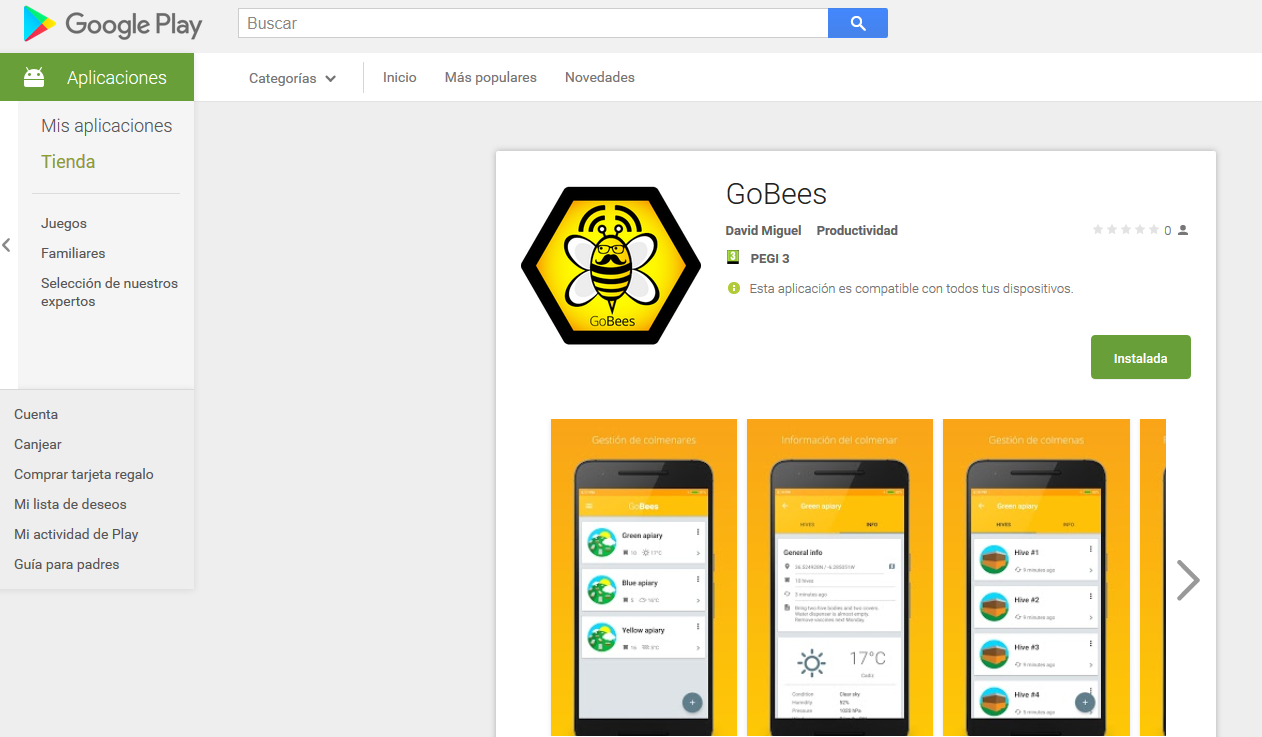
\includegraphics[width=0.65\textwidth]{gobees-google-play}
	\caption{GoBees en Google Play.}\label{fig:gobees-google-play}
\end{figure}

Además, se desarrolló una página web promocional
(\href{http://gobees.io/}{gobees.io}), donde se describen las
características de la aplicación, los manuales de usuario, y el enlace
de descarga, entre otras cosas.

Por último, se crearon perfiles en las principales redes sociales para
promocionar la aplicación.

\section{Reconocimientos}\label{reconocimientos}

Durante el desarrollo del proyecto se obtuvieron varios reconocimientos:

\begin{itemize}
\tightlist
\item
  \textbf{Beca de colaboración con departamentos}: se me concedió esta
  beca para profundizar en el algoritmo desarrollado y publicar un
  artículo científico sobre él.
\item
  \textbf{Prototipos Orientados al Mercado}: GoBees resultó ganador de
  uno de los tres premios de la convocatoria de Prototipos Orientados al
  Mercado realizada por el Vicerrectorado de Investigación y
  Transferencia del Conocimiento~de la Universidad de Burgos.
\item
  \textbf{YUZZ}: GoBees fue elegido para participar en el programa YUZZ
  2017, patrocinado por el Banco Santander para el impulso del talento
  joven y el espíritu emprendedor.
\end{itemize}

\capitulo{6}{Trabajos relacionados}

Como se comentó en la introducción, los intentos de automatizar el
proceso de monitorización de la actividad de una colmena se remontan
hasta principios del siglo pasado. Sin embargo, no es hasta 2008 cuando
se introduce la visión artificial en este campo. A continuación, se
exponen los artículos científicos relacionados publicados hasta la
fecha, así como proyectos con objetivos similares.

\section{Artículos científicos}\label{artuxedculos-cientuxedficos}

\subsection{Video Monitoring of Honey Bee Colonies at the Hive
Entrance}\label{video-monitoring-of-honey-bee-colonies-at-the-hive-entrance}

Se trata del primer artículo publicado sobre el tema (año 2008). Los
autores fueron Jason Campbell, Lily Mummert y Rahul Sukthankar del
\emph{Intel Research Pittsburgh}. En él proponen un método de visión
artificial para monitorizar las entradas y salidas de abejas en una
colmena, consiguiendo diferenciar las que entran de las que salen. Se
describen los desafíos técnicos que supuso y la solución a la que
llegaron finalmente \citep{art:campbell2008}.

\subsection{Detecting and tracking honeybees in 3D at the beehive
entrance using stereo
vision}\label{detecting-and-tracking-honeybees-in-3d-at-the-beehive-entrance-using-stereo-vision}

En 2013, Guillaume Chiron, Petra Gomez-Krämer y Ménard Michel publicaron
un artículo en \emph{EURASIP Journal on Image and Video Processing,}
donde proponían un método para la monitorización de abejas a la entrada
de una colmena basado en un sistema de tiempo real con visión
estereoscópica. Gracias al cual podían obtener una representación en
tres dimensiones de las trayectorias de las abejas
\citep{art:chiron2013}.

\subsection{Image Processing for Honey Bee hive Health
Monitoring}\label{image-processing-for-honey-bee-hive-health-monitoring}

El último artículo publicado data del año 2015 por Rahman Tashakkori y
Ahmad Ghadiri de la \emph{Appalachian State University}. En él, mejoran
el método de detección propuesto en \citep{art:campbell2008} y lo
utilizan para estimar el número de abejas que habrá en un instante de
tiempo dado \citep{art:tashakkori2015}.

\subsection{Comparativa sobre las técnicas utilizadas}\label{comparacion-articulos}

A continuación, se muestran las diferentes técnicas de detección de movimiento,
conteo de abejas y \emph{tracking} utilizadas en los tres artículos 
anteriores y se comparan con las utilizadas en el proyecto.

\tablaSmall{Comparativa métodos de detección de movimiento.}{l l l l l}{comparativa-1}
{ Artículo & Año & Citas & Detección de movimiento \\}{ 
{\citep{art:campbell2008}}   & 2008 & 24 & \emph{Adaptative background subtraction}. \\
{\citep{art:chiron2013}}     & 2013 & 8  & \specialcell{\emph{Adaptative background subtraction}\\\emph{with depth information}.} \\
{\citep{art:tashakkori2015}} & 2015 & 0  & \specialcell{\emph{Averaging a background with}\\\emph{illumination invariant method}.}\\
GoBees                       & 2017 & 0  & \specialcell{\emph{Mixture of Gaussians method}\\(\texttt{BackgroundSubtractorMOG2}).}     \\
} 

\tablaSmall{Comparativa métodos de conteo de abejas y \emph{tracking}.}{l l l}{comparativa-2}
{ Artículo & Conteo de abejas & \emph{Tracking} \\}{ 
{\citep{art:campbell2008}} & \emph{Template-based method.} & \specialcell{\emph{Maximum weighted bipartite}\\\emph{graph matching.}} \\
{\citep{art:chiron2013}} & \specialcell{\emph{Hybrid 3D intensity}\\\emph{depth method.}} & \specialcell{\emph{Kalman filter }y\\\emph{Global Nearest Neighbor}.} \\
{\citep{art:tashakkori2015}} & \emph{Area-based method.} & No \\
GoBees & \emph{Area-based method.} & No \\
} 
\newpage

\section{Proyectos}\label{proyectos}

\subsection{EyesOnHives}\label{eyesonhives}

EyesOnHives es el principal competidor del proyecto. Se trata de un
producto comercial cuyo fin es la monitorización del estado de salud de
las colmenas mediante su actividad de vuelo. Integra un \emph{hardware}
específico que se encarga de la captación de imágenes y una plataforma
en la nube que las procesa y permite el acceso a los datos.

\begin{itemize}
\tightlist
\item
  Web del proyecto: \url{http://www.keltronixinc.com}
\end{itemize}

\subsection{HiveTool}\label{hivetool}

Se trata de un proyecto \emph{OpenSource} que ofrece un conjunto de
herramientas para monitorizar distintos parámetros de una colmena. Una
de estas herramientas es ``Bee Counter'', un contador de abejas por
visión artificial desarrollado sobre una Raspberry Pi.

\begin{itemize}
\tightlist
\item
  Web del proyecto: \url{http://hivetool.org}
\end{itemize}

\section{Fortalezas y debilidades del
proyecto}\label{fortalezas-y-debilidades-del-proyecto}

\begin{table}[H]
\centering
\begin{tabular}{lccc}
\toprule
Características                 & GoBees     & EyesOnHives & HiveTool   \\
\midrule
No requiere \emph{hardware} específico & \cellcolor{green!25} {$\checkmark$} & \cellcolor{red!25} {$\times$} & \cellcolor{red!25} {$\times$} \\
Instalación sencilla            & \cellcolor{green!25} {$\checkmark$} & \cellcolor{green!25} {$\checkmark$}  & \cellcolor{red!25} {$\times$} \\
Procesamiento en local          & \cellcolor{green!25} {$\checkmark$} & \cellcolor{yellow!25} Parcial & \cellcolor{green!25} {$\checkmark$}  \\
No requiere \emph{wifi}         & \cellcolor{green!25} {$\checkmark$} & \cellcolor{red!25} {$\times$} & \cellcolor{green!25} {$\checkmark$}  \\
No requiere red eléctrica       & \cellcolor{green!25} {$\checkmark$} & \cellcolor{red!25} {$\times$}  & \cellcolor{green!25} {$\checkmark$}  \\
Localización GPS                & \cellcolor{green!25} {$\checkmark$} & \cellcolor{red!25} {$\times$} & \cellcolor{red!25} {$\times$}        \\
Gratuito                        & \cellcolor{green!25} {$\checkmark$} & \cellcolor{red!25} {$\times$}  & \cellcolor{green!25} {$\checkmark$}  \\
Plataformas                     & Android    & Web App     & Linux     \\
\bottomrule
\end{tabular}
\caption{Comparativa de las características de los proyectos.}
\label{comparativa-proyectos}
\end{table}

Las principales fortalezas del proyecto son:

\begin{itemize}
\tightlist
\item
  No se necesita adquirir ningún \emph{hardware} específico como en el
  resto de proyectos, simplemente se necesita un \emph{smartphone} con
  Android. Esto hace el proyecto mucho más accesible a los potenciales
  usuarios.
\item
  La instalación es muy sencilla. Únicamente se requiere un trípode o
  cualquier otro tipo de soporte que permita sujetar el
  \emph{smartphone} en posición cenital.
\item
  El procesamiento de las imágenes se realiza en local no en un
  servidor. Considerando que los colmenares suelen estar en medio del
  monte, no podemos requerir una conexión \emph{wifi} como necesita
  EyesOnHives y el envío de vídeo mediante tecnologías 3G/4G supondría
  un coste económico muy elevado.
\item
  No requiere estar conectado a la red eléctrica. El \emph{smartphone}
  cuenta con su propia batería. El consumo de la aplicación no es muy
  elevado al estar la pantalla apagada durante la monitorización. Aun
  así, se pueden utilizar \emph{powerbanks} (baterías portátiles) en
  caso de ser necesarios.
\item
  El \emph{smartphone} tiene integradas varias tecnologías de
  transmisión de información. Lo da la posibilidad de crear una
  plataforma que centralice la recogida de datos de varios dispositivos
  sin importar su localización.
\item
  Relacionado con el punto anterior, el \emph{smartphone} nos permite
  estar conectados a internet, posibilitándonos ampliar la información
  que maneja nuestra aplicación. Por ejemplo, podemos acceder a la
  información meteorológica en tiempo real.
\item
  El GPS del \emph{smartphone} nos permite localizar geográficamente la
  monitorización y, por tanto, la información meteorológica. Además,
  puede ser de utilidad en caso de robo, gracias a aplicaciones como
  \emph{Android Device Manager}, Cerberus, etc. que permiten localizar
  el dispositivo de forma remota.
\end{itemize}

Las principales debilidades son:

\begin{itemize}
\tightlist
\item
  Actualmente solo se encuentra disponible para Android. Aunque en una
  segunda fase del proyecto se creará una plataforma en la nube que
  centralice todos los datos y una aplicación web que permita acceder a
  ellos.
\item
  El utilizar un \emph{smartphone} como soporte \emph{hardware} tiene
  sus ventajas, pero también sus inconvenientes. La cámara no tiene el
  mismo rendimiento que una cámara diseñada específicamente para esta
  tarea. Esto nos ha limitado en las técnicas de visión artificial que
  hemos podido aplicar, por no disponer de imágenes con la suficiente
  nitidez.
\end{itemize}

\capitulo{7}{Conclusiones y Líneas de trabajo futuras}

En esta sección se exponen las conclusiones derivadas del trabajo, así
como las posibles líneas de trabajo futuras por las que se puede dar
continuidad al proyecto.

\section{Conclusiones}\label{conclusiones}

Tras el desarrollo del proyecto podemos extraer las siguientes
conclusiones:

\begin{itemize}
\tightlist
\item
  El objetivo general del proyecto se ha cumplido satisfactoriamente.
  Ahora los apicultores cuentan con una aplicación Android que no solo
  les permite gestionar sus colmenares, sino que además les brinda la
  posibilidad de monitorizar la actividad de vuelo de sus colmenas e
  interpretar los datos recogidos.
\item
  El haber utilizado el ecosistema Android para la realización del
  proyecto ha aportado ciertas ventajas tanto en herramientas de
  desarrollo, como en la distribución de la aplicación. Sin embargo,
  también ha supuesto un desafío al tener que desarrollar un algoritmo
  de una cierta complejidad para dispositivos con recursos bastante
  limitados.
\item
  El proyecto ha abarcado gran parte de los conocimientos adquiridos
  durante el grado. Además, ha requerido el aprendizaje de muchos otros
  como la visión artificial, OpenCV, Android, etc.
\item
  Durante el proyecto se han utilizado un gran número de tecnologías y
  herramientas. La mayoría de ellas han contribuido a mejorar la calidad
  del producto final o de los procesos intermedios. No obstante, algunas
  de ellas han supuesto una sobrecarga importante, como sucedió en el
  caso de la documentación. Aun así, el conocimiento adquirido de todas
  ellas será de mucha utilidad en proyectos futuros.
\item
  Gracias a la parte de investigación que posee el proyecto, se ha
  aprendido a realizar búsquedas bibliográficas y a familiarizarse con
  la lectura de artículos científicos.
\item
  La utilización de varios servicios de integración continua nos ha
  permitido la detección temprana de defectos en el \emph{software},
  reduciendo el impacto de estos y dando lugar a un código de mayor
  calidad.
\item
  Es muy difícil estimar la duración de tareas de investigación o tareas
  sobre las que no se posee un conocimiento previo. Sin embargo, el
  haber aplicado una metodología ágil nos ha permitido ser más flexibles
  ante los cambios. Y finalmente, se ha completado satisfactoriamente el
  proyecto en el plazo establecido.
\end{itemize}

\section{Líneas de trabajo futuras}\label{luxedneas-de-trabajo-futuras}

En primer lugar, comentar que la entrega del Trabajo de Fin de Grado
solo es un hito en el camino del proyecto, ya que su desarrollo
prosigue. A continuación, se resume el \emph{roadmap} del proyecto:

\begin{itemize}
\tightlist
\item  En la columna ``\emph{New issues}'' del gestor de tareas se encuentran
  las nuevas funcionalidades en las que se trabajarán en los próximos
  meses. Entre ellas se encuentran: dar soporte a operaciones por lotes
  orientadas a apicultores profesionales con un gran número de colmenas,
  permitir la exportación de los datos almacenados, añadir informes de
  revisión de colmenas, varias mejoras de usabilidad y diseño, etc.
\item
  Por otro lado, para la beca de colaboración con departamentos se
  trabajará en la mejora del algoritmo de monitorización actual. Se
  probarán nuevas técnicas de detección y \emph{tracking}, y se
  estudiará su viabilidad para ser ejecutadas en dispositivos móviles.
\item
  Para finales de año se planea tener desarrollada una plataforma en la
  nube que sincronice los datos de varios dispositivos y permita el
  acceso a estos mediante una aplicación web. Se planea monetizar el
  proyecto mediante la subscripción a esta plataforma.
\item
  Se considerará la opción de migrar la aplicación a otras plataformas.
\item
  En el futuro, se podrían explotar los datos almacenados en la
  plataforma para intentar desarrollar algoritmos que predigan ciertos
  eventos (enfermedades, enjambrazón, etc.) y que permitan al apicultor
  anticiparse a estos.
\end{itemize}



\bibliography{bibliografia}
\bibliographystyle{plainnat}

\end{document}